\documentclass{article}[11pt]
\usepackage[frenchb,english]{babel}
\usepackage[T1]{fontenc}
\usepackage[utf8]{inputenc}
\usepackage{amsmath,amssymb,latexsym}
\usepackage{times}
\usepackage{float}
\usepackage[left=2cm,right=2cm,top=2cm,bottom=2cm]{geometry}
\frenchbsetup{StandardLists=true} % � inclure si on utilise \usepackage[french]{babel}
\usepackage{enumitem}
\usepackage{fancyhdr}
\usepackage{mathrsfs}
\usepackage{graphicx}
%\usepackage[Algorithme]{algorithm}
%\usepackage{algorithmic}
\usepackage{tikz}
\usepackage{tabularx}
\usetikzlibrary{shapes}
\pagestyle{fancy}
\newcommand{\tr}[1]{{\vphantom{#1}}^{\mathit t}{#1}} 
\renewcommand\headrulewidth{1pt}
\fancyhead[L]{Cours 1�re S}
\fancyhead[R]{Yoann Pietri}
\newcounter{theoremecounter}[subsection]
\usepackage{titlesec}
\setcounter{secnumdepth}{3}% enl�ve la num�rotation apr�s les sections
%\renewcommand\thechapter {\Roman{chapter}}

 \setlength{\parindent}{0pt}

\newcommand{\R}{\mathbb{R}}
\newcommand{\N}{\mathbb{N}}
\newcommand{\Q}{\mathbb{Q}}
\newcommand{\Z}{\mathbb{Z}}
\newcommand{\C}{\mathbb{C}}
\newcommand{\K}{\mathbb{K}}
\newcommand{\eqi}{\Leftrightarrow}
\titleformat{\subsubsection}
   {\normalfont\fontsize{11pt}{13pt}\selectfont\bfseries}% apparence commune au titre et au num�ro
   {\thesubsubsection}% apparence du num�ro
   {1em}% espacement num�ro/texte
   {}% apparence du titre

\tikzstyle{theobox} = [draw=black, very thick,
    rectangle, rounded corners, inner sep=10pt, inner ysep=20pt]
\tikzstyle{theotitle} =[fill=white, text=black,rounded corners,draw=black,very thick]

\fancyhead[L]{Contrôle chapitre 1}

\usepackage{tkz-tab}

\begin{document}
\center
\Large Contrôle de cours (correction)
\flushleft
\center
Trinômes du second degré 
\flushleft \normalsize
\subsection*{Exercice 1 (R.O.C., temps conseillé : 10 min) : }
Soit $f$ une fonction trinôme 
$$f(x) = ax^2 + bx + c$$ 
$a\neq 0$. On suppose de plus que pour tout $x\in \R$, $$f(x) = a'x^2 +b'x +c'$$ Alors, on a $$f(0) = c$$ et $$f(0) = c'$$ donc $$c=c'$$ De plus $$f(1) = a+b = a'+b'$$ $$f(-1) = a-b = a'-b'$$Le système $$\left\{\begin{array}{l} a+b =a' +b'\\a-b=a'-b'\end{array} \right.$$ devient (en sommant les deux lignes par exemple) $$\left\{\begin{array}{l} a =a'\\b=b'\end{array} \right.$$

Toute fonction trinôme $f(x) = ax^2+bx+c$ avec $a\neq0$ s'écrit $$f(x) = a\left(x+\frac{b}{2a}\right)^2 - \frac{\Delta}{4a}$$ où $\Delta = b^2 -4ac$\newline

L'équation $$f(x) = 0$$ est équivalente à $$\left(x+\frac{b}{2a}\right)^2 = \frac{\Delta}{4a^2}$$ d'après le résultat sur les formes canoniques. Ainsi, si $\Delta > 0$, le trinôme admet deux racines qui vérifient $$x_{1,2} + \frac{b}{2a} = \pm\frac{\sqrt{\Delta}}{2a}$$ d'ou $$x_{1,2} = \frac{-b \pm \sqrt{\Delta}}{2a}$$ Si $\Delta =0$, le trinôme a une unique racine : $$x_0 = -\frac{b}{2a}$$ et si $\Delta < 0$, le trinôme n'a pas de racines réelles
\subsection*{Exercice 2 (Etude d'une fonction trinôme, temps conseillé : 15 min) : }
On considère la fonction $f$ définie pour tout $x$ par $$f(x) = 2x^2-5x-3$$
\begin{enumerate}
\item $f$, comme toutes les fonctions trinômes, est définie sur $\R$
\item $$f(1) = 2\times(1)^2 - 5\times 1 - 3 = -6$$ 
$$\boxed{f(1) = -6}$$
$$f(4) = 2\times 16 -5\times4-3 = 9$$ $$\boxed{f(4) = 9}$$ et $$f(-1) = 2\times(-1)^2 + 5 -3 = 4$$
$$\boxed{f(-1) = 4}$$
\item On utilise le résultat sur les formes canoniques avec $a=2$, $b=-5$ et $c= -3$. On calcule tout d'abord le discriminant : 
$$\delta = (-5)^2 -4\times2\times(-3) = 25 + 24 = 49$$
Ainsi 
$$f(x) = 2\left(x+\frac{-5}{2\times2}\right)^2 -\frac{49}{4\times2}$$
$$\boxed{f(x) = 2\left(x-\frac{5}{4}\right)^2 - \frac{49}{8}}$$
\item D'après la question précédente $$\delta = 49 > 0$$ donc ce trinôme admet 2 racines réelles distinctes qui sont $$x_1 = \frac{5 - \sqrt{49}}{2\times 2} = \frac{5-7}{4}$$$$\boxed{x_1 = -\frac{1}{2}}$$ $$x_2 = \frac{5 + \sqrt{49}}{2\times 2} = \frac{5+7}{4}$$$$\boxed{x_2 = 3}$$
\item On a $$f(x) = a(x-x_1)(x-x_2)$$
$$\boxed{f(x) = 2\left(x+\frac{1}{2}\right)\left(x-3\right)}$$
\item Le coefficient dominant de $f$ est positif donc $f$ est négatif entre ses racines. Ainsi \newline

\begin{tikzpicture}
   \tkzTabInit{$x$ / 1 , $f(x)$ / 1}{$-\infty$,$-\frac{1}{2}$,$3$, $+\infty$}
   \tkzTabLine{, +,z,-,z, +,}
\end{tikzpicture}
\item Voici la représentation graphique de $f$ : \newline

\center
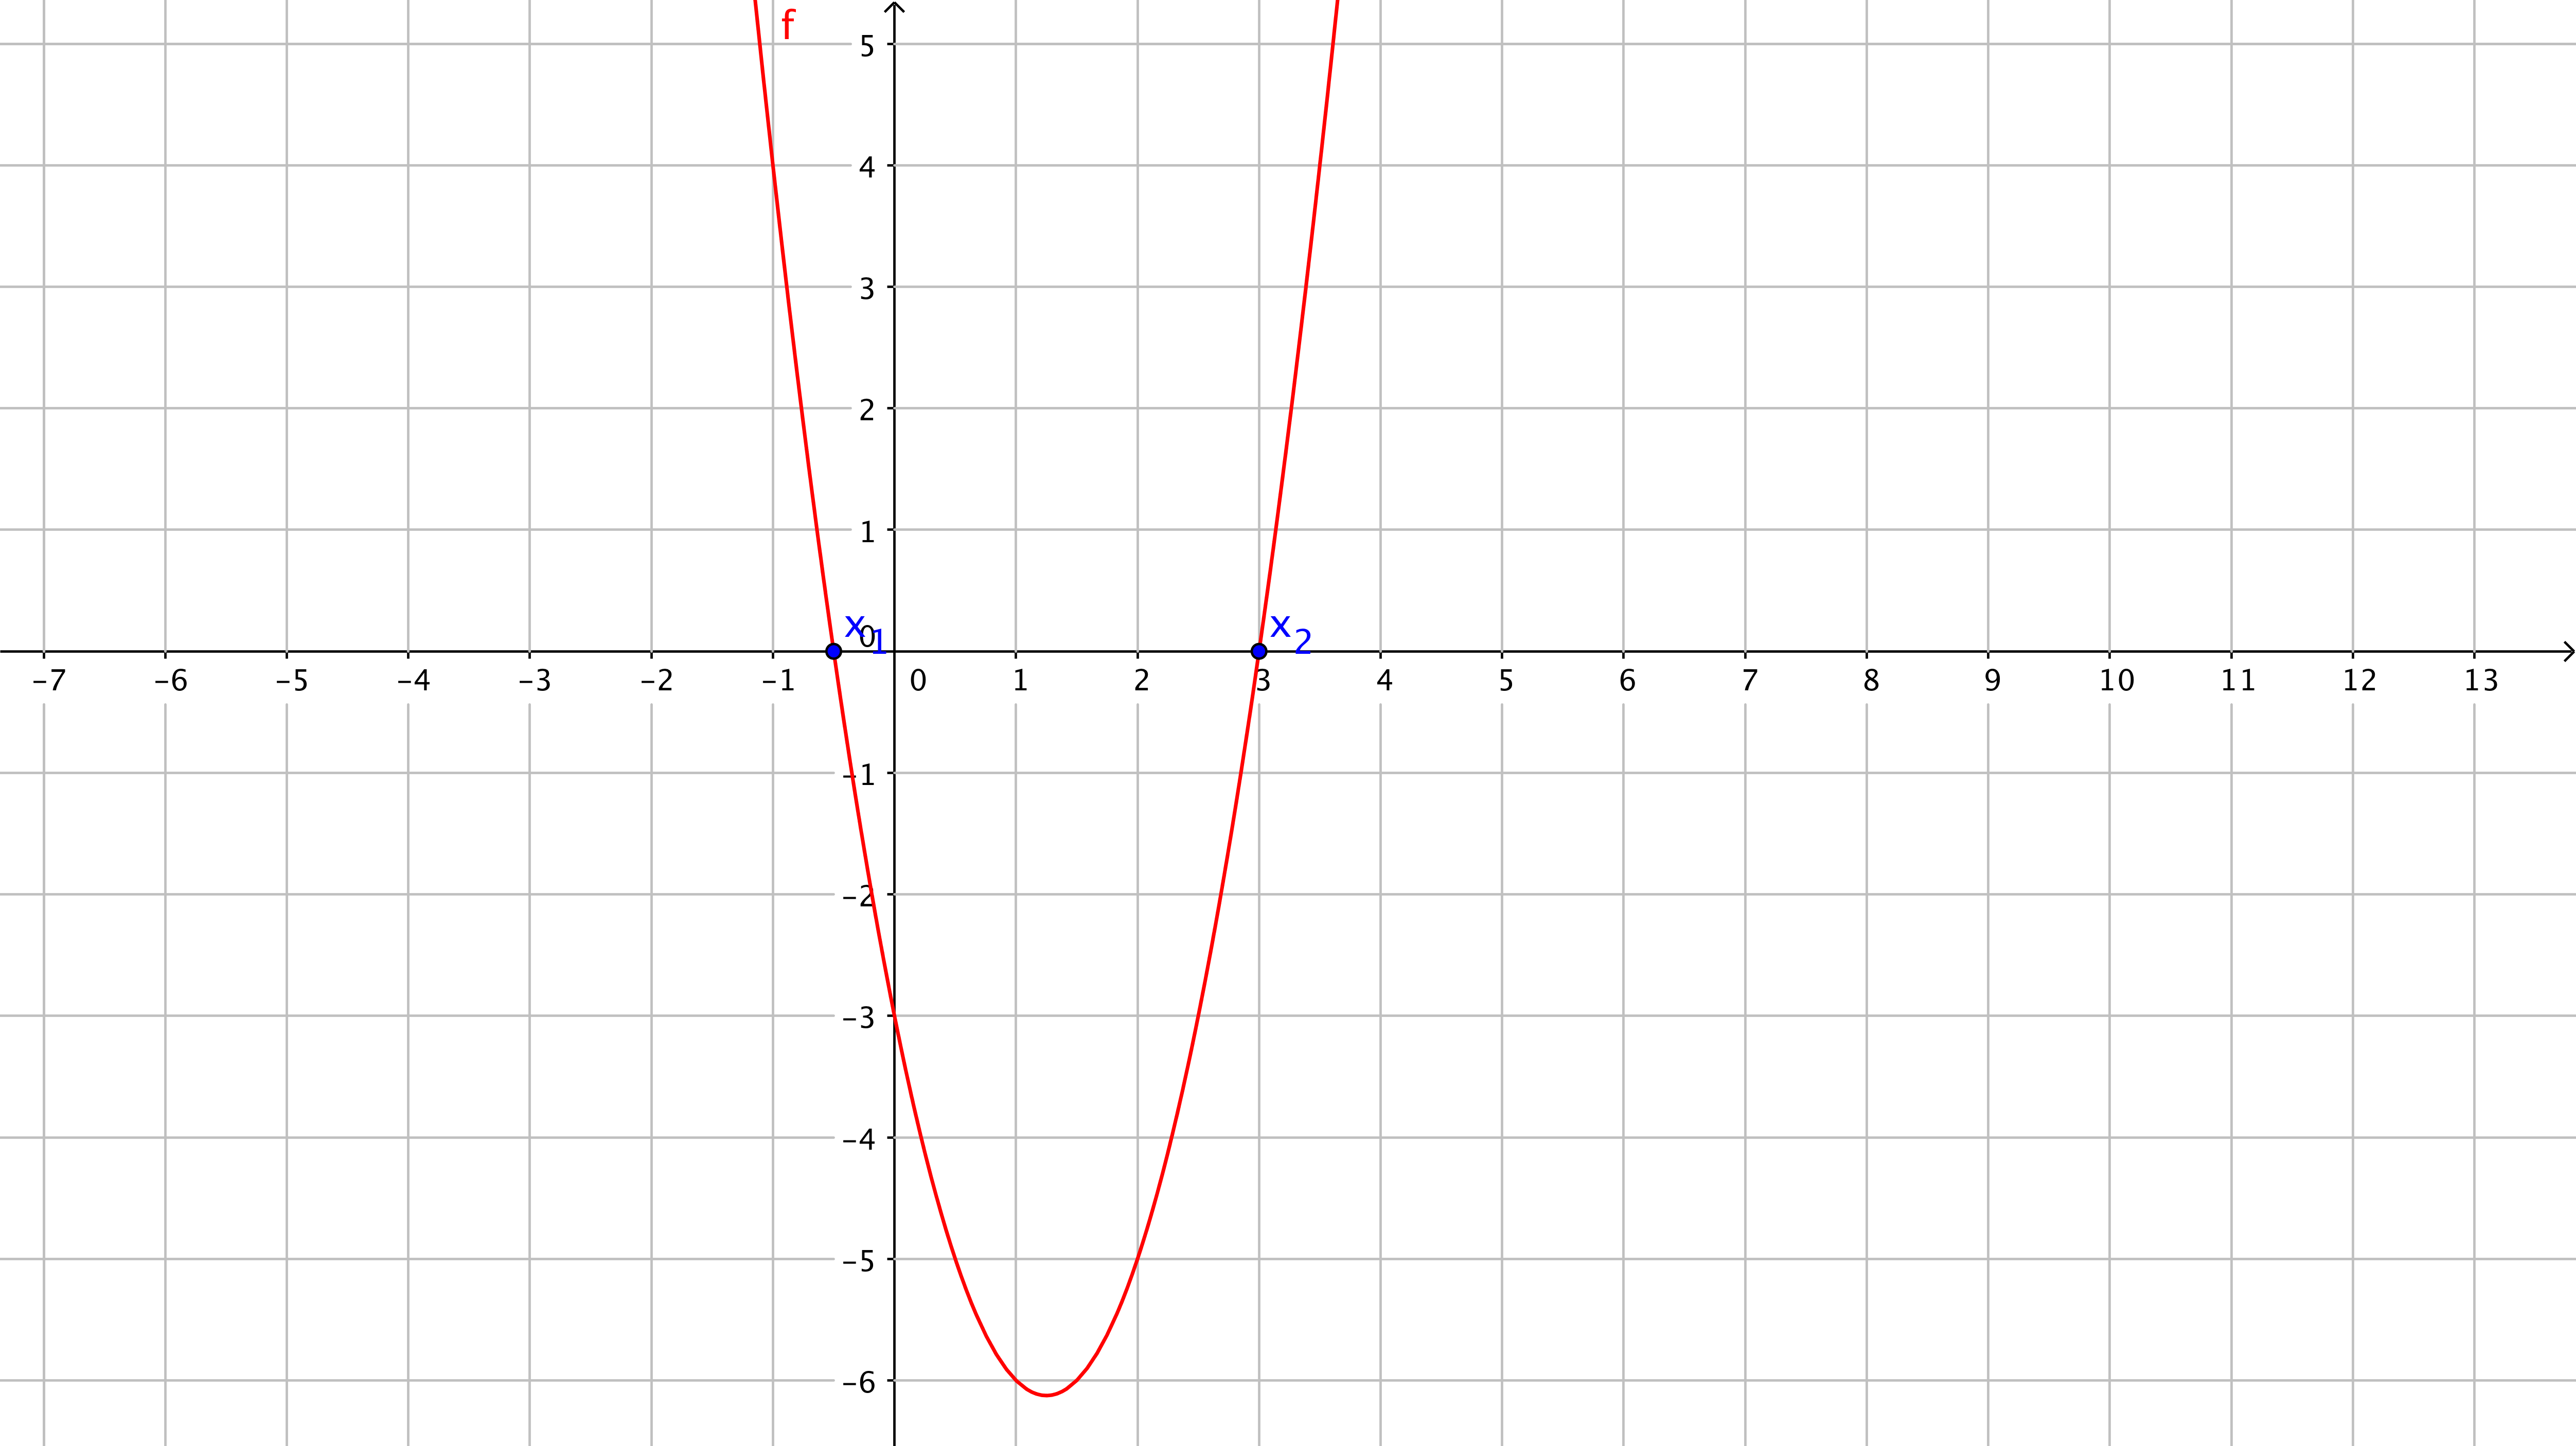
\includegraphics[scale=0.7]{chap1_corr_ill1.png}
\flushleft
\end{enumerate}
\subsection*{Exercice 3 (Equation et inéquation du second degré, temps conseillé : 15 min) : }
\begin{enumerate}
\item On a 
$$2x^2 + 7 x -1 = 1 - x^2 + 2x$$
$$\Leftrightarrow 3x^2 +5x -2 = 0$$ 
On calcule le discriminant de ce trinôme : 
$$\Delta = 5^2 + 4\times 3 \times 2 = 49$$
On a $\Delta > 0$ donc ce trinôme admet deux racines distinctes qui sont
$$x_1 = \frac{-5 - \sqrt{49}}{2\times 3} = \frac{-5-7}{6} = -2$$
$$x_2 = \frac{-5 + \sqrt{49}}{2\times 3} = \frac{-5+7}{6} = \frac{1}{3}$$
Ainsi, l'ensemble des solutions de cette équation est 
$$\boxed{\mathcal{S} = \left\{-2;\frac{1}{3}\right\}}$$
\item On a
$$x\left(\frac{1}{2}x + \frac{3}{2}\right) < 2$$
$$\Leftrightarrow x\left(x + 3\right) < 4\quad (\text{Multiplication par 2 des deux cotés de l'inégalité})$$
$$\Leftrightarrow x^2 + 3x -4 < 0$$
On établit le tableau de signe de ce trinôme : on commence par calculer le discriminant : 
$$\Delta = 3^2 +4\times 4 = 9 +16 = 25$$
$\Delta > 0$ donc ce trinôme admet 2 solutions réelles distinctes qui sont 
$$x_1 = \frac{-3-\sqrt{25}}{2\times1} = \frac{-8}{2} = -4$$
$$x_2 = \frac{-3+\sqrt{25}}{2\times1} = \frac{2}{2} = 1$$
Le coefficient dominant de ce trinôme est positif donc le trinôme est négatif entre les racines. Ainsi l'intervalle solution est 
$$\boxed{\mathcal{S} = ]-4,1[}$$
Si des difficultés, regarder le tableau de signe : \newline

\begin{tikzpicture}
   \tkzTabInit{$x$ / 1 , $x^2+3x-4$ / 1}{$-\infty$,$-4$,$1$, $+\infty$}
   \tkzTabLine{, +,z,-,z, +,}
\end{tikzpicture}
\end{enumerate}
\subsection*{Exercice 4 (Symétries, temps conseillé : 15-20 min) : }
On considère la fonction $f$ définie pour tout $x\in \R$ par 
$$f(x) = ax^2+bx+c$$
avec $a\neq 0$
\begin{enumerate}
\item On a $$ f\left(-\frac{b}{2a}\right) = a\left(-\frac{b}{2a}\right)^2 + b\left(-\frac{b}{2a}\right) + c$$
$$f\left(-\frac{b}{2a}\right) = \frac{b^2}{4a} - \frac{b^2}{2a} + c$$
$$f\left(-\frac{b}{2a}\right) = \frac{b^2}{4a} - 2\frac{b^2}{4a} + c$$
$$\boxed{f\left(-\frac{b}{2a}\right) = - \frac{b^2}{4a} + c}$$
Si l'on inclut le $c$ dans la fraction, 
$$\boxed{f\left(-\frac{b}{2a}\right) = \frac{-b^2 + 4ac}{4a} = -\frac{\Delta}{4a}}$$
On vit alors le lien avec la forme canonique
\item $$f(x)- f\left(-\frac{b}{2a}\right) = \left(a\left(x+\frac{b}{2a}\right)^2 -\frac{\Delta}{4a}\right) - \frac{-\Delta}{4a}$$
$$f(x)- f\left(-\frac{b}{2a}\right) = a\left(x+\frac{b}{2a}\right)^2 -\frac{\Delta}{4a} + \frac{\Delta}{4a}$$
$$\boxed{f(x)- f\left(-\frac{b}{2a}\right) = a\left(x+\frac{b}{2a}\right)^2}$$
\item Le terme $\displaystyle \left(x+\frac{b}{2a}\right)^2$ est tout le temps positif. Ainsi si $a > 0$, on a pour tout $x$, 
$$f(x)- f\left(-\frac{b}{2a}\right) \geq 0$$ donc $$\boxed{f(x) \geq f\left(-\frac{b}{2a}\right)}$$ d'où l'on déduit que c'est un minimum et si $a<0$, on a pour tout $x$ $$f(x)- f\left(-\frac{b}{2a}\right) \leq 0$$ donc $$\boxed{f(x) \leq f\left(-\frac{b}{2a}\right)}$$ d'où l'on déduit que c'est un maximum
\item 
$$f\left(-\frac{b}{2a} - x\right) = a\left(-\frac{b}{2a} - x\right)^2 + b\left(-\frac{b}{2a} +x\right) + c$$
$$f\left(-\frac{b}{2a} - x\right) = a\left(\frac{b}{2a} + x\right)^2 - b\left(\frac{b}{2a} +x\right) +c$$
$$f\left(-\frac{b}{2a} - x\right) = a\left(\frac{b^2}{4a^2} + 2\frac{b}{2a}x + x^2\right) - \frac{b^2}{2a} - bx +c$$
$$f\left(-\frac{b}{2a} - x\right) = \frac{b^2}{4a} + bx + ax^2 - \frac{b^2}{2a} -bx +c$$
$$\boxed{f\left(-\frac{b}{2a} - x\right) = -\frac{b^2}{4a} + ax^2 +c}$$

$$f\left(-\frac{b}{2a} + x\right) = a\left(-\frac{b}{2a} -+x\right)^2 + b\left(-\frac{b}{2a} +x\right) + c$$
$$f\left(-\frac{b}{2a} + x\right) = a\left(\frac{b^2}{4a^2} - 2\frac{b}{2a}x + x^2\right) - \frac{b^2}{2a} + bx +c$$
$$f\left(-\frac{b}{2a} + x\right) = \frac{b^2}{4a} - bx + ax^2 - \frac{b^2}{2a} +bx +c$$
$$\boxed{f\left(-\frac{b}{2a} - x\right) = -\frac{b^2}{4a} + ax^2 +c}$$

On déduit 
$$\boxed{f\left(-\frac{b}{2a} - x\right) = f\left(-\frac{b}{2a} +x\right)}$$
La conséquence est que la courbe représentative de $f$ est symétrique par rapport à la droite d'équation $x=-\frac{b}{2a}$
\item On a tracé la courbe représentative de $x\mapsto x^2-x-1$ et la droite d'équation $x=\frac{1}{2}$. \newline

\center
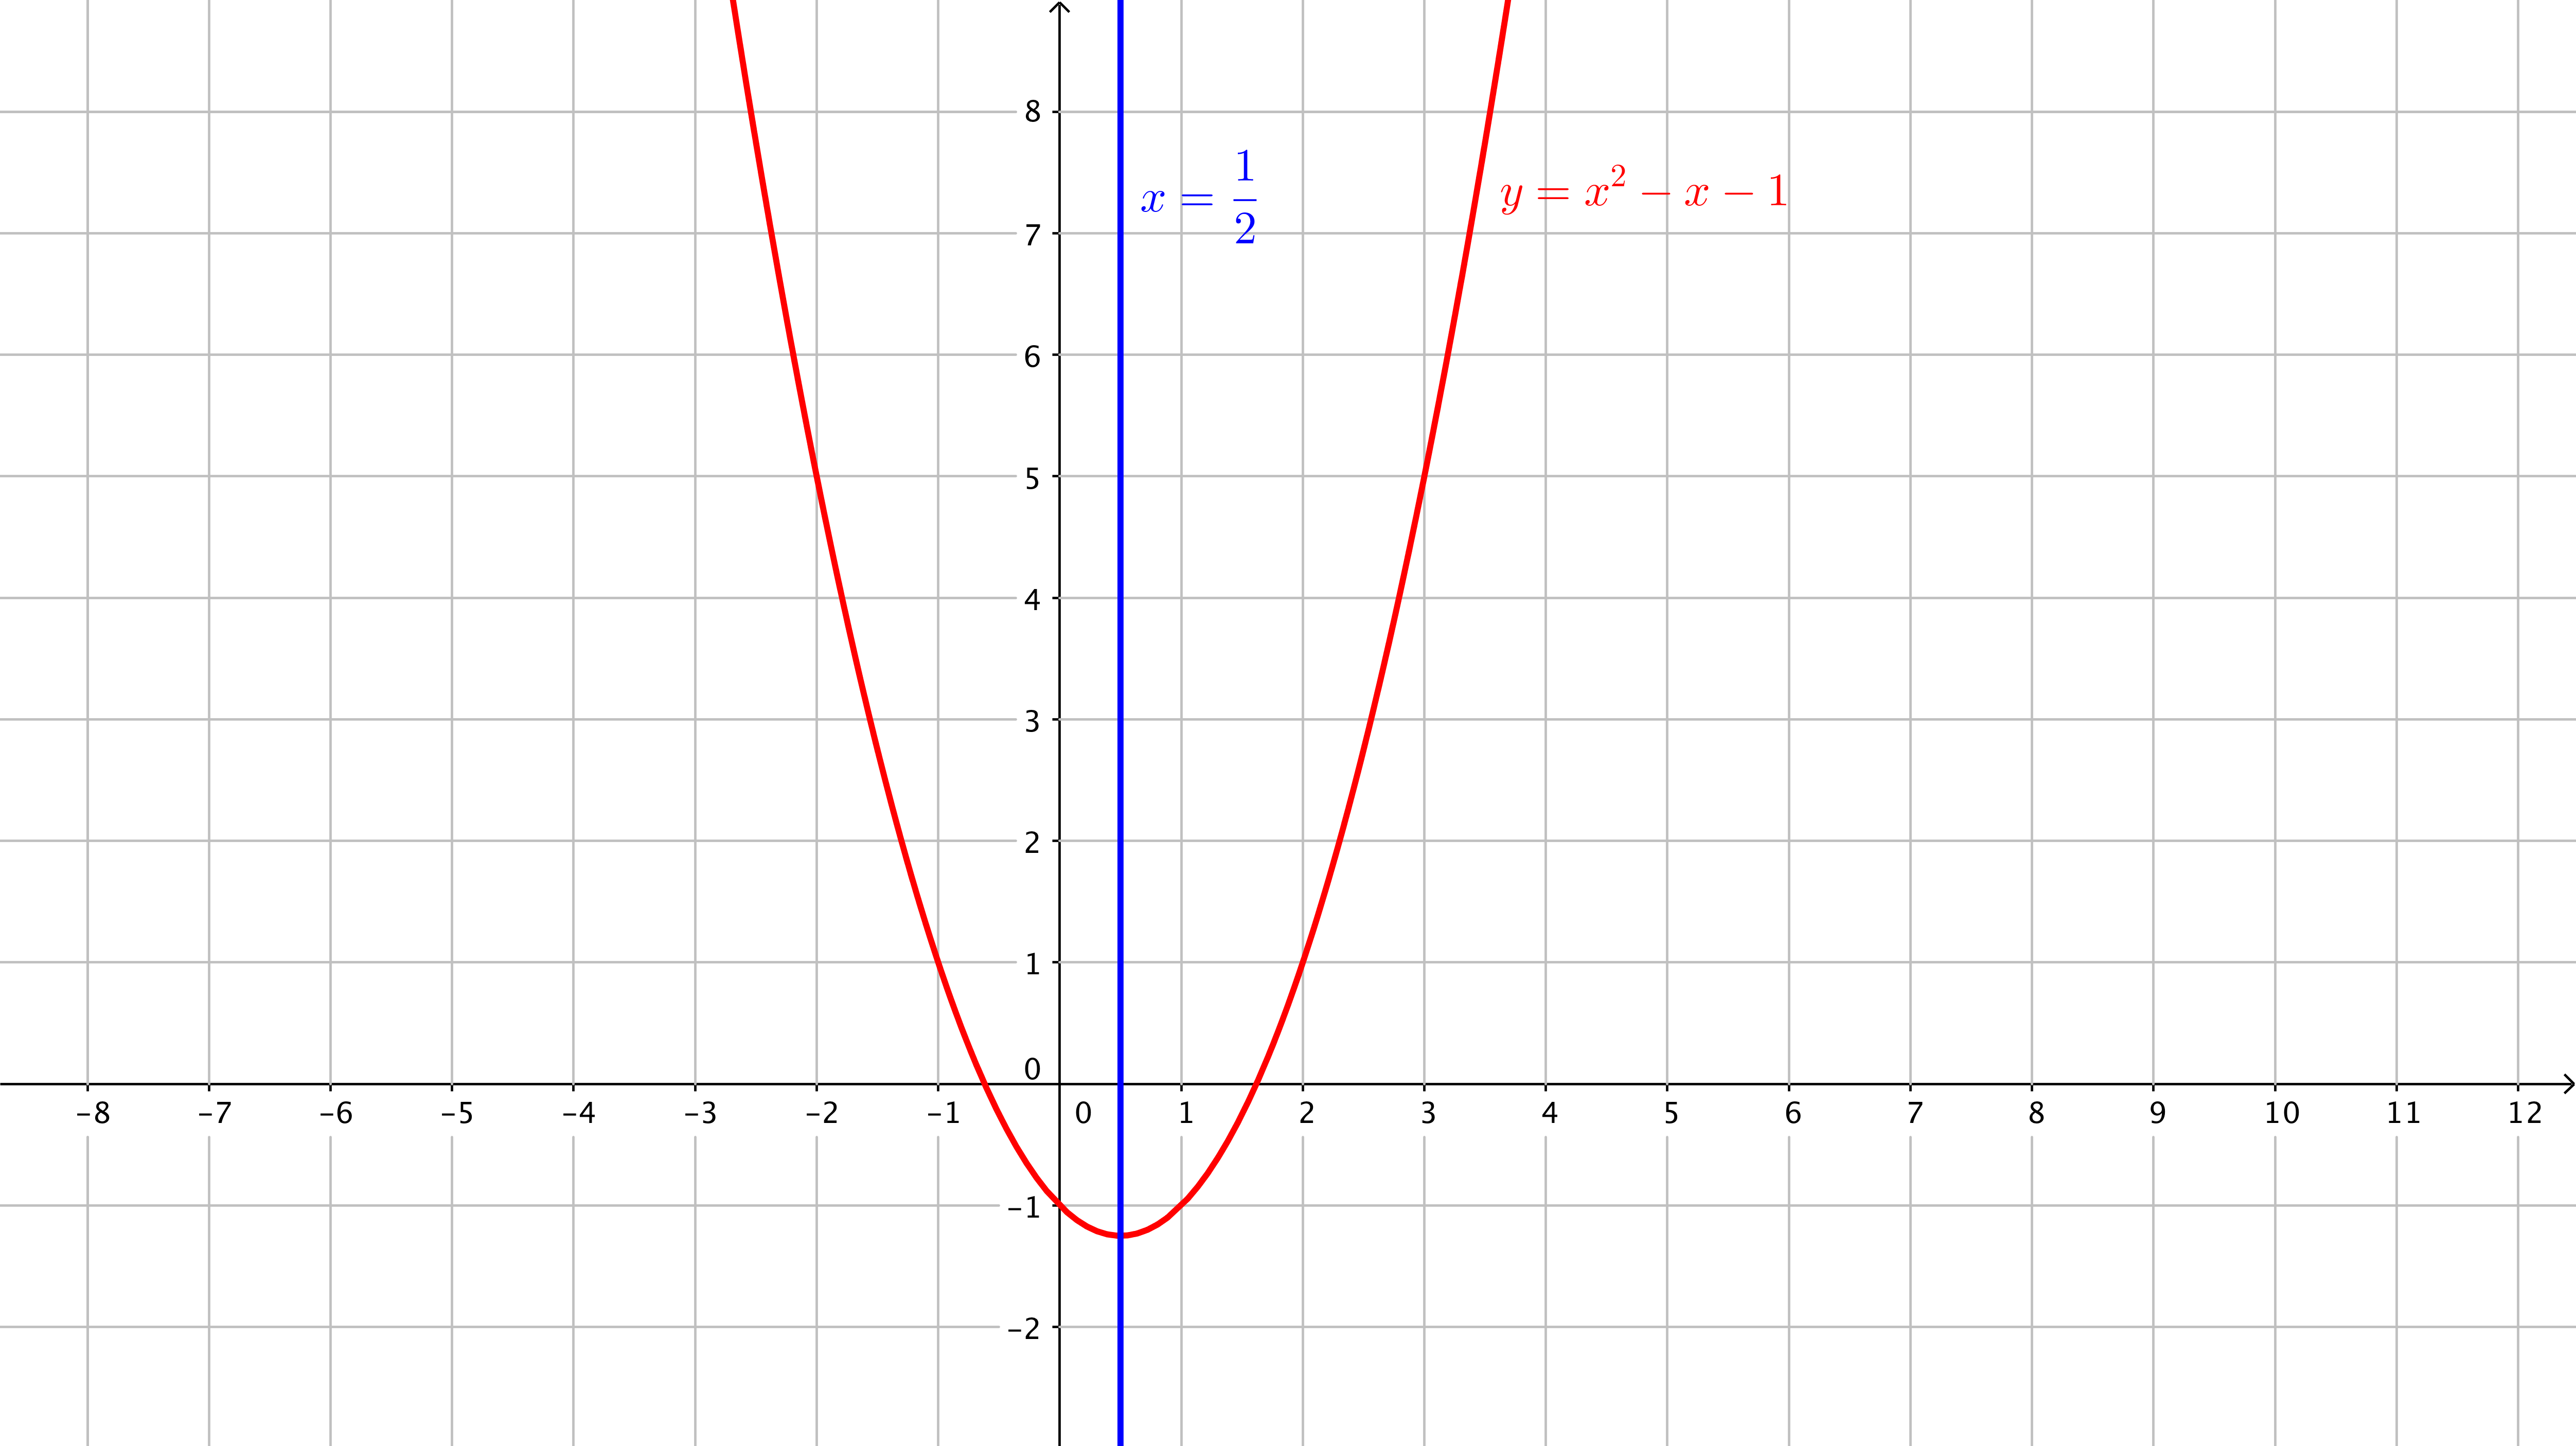
\includegraphics[scale=0.7]{chap1_corr_ill2.png}
\flushleft
On remarque bien la symétrie
\end{enumerate}
$$\star \star \star$$
\center
FIN DU SUJET
\end{document}